\documentclass[../main.tex]{subfiles}
\graphicspath{{./images/}}

\begin{document}

\section{Methodology and tooling} \label{sec:methodology_and_tooling}
This section explains the high-level aspects regarding the self-imposed  methodology, assumptions and requirements that are taken to narrow down the reach of the project. That is, what are the conditions under which the object detection task is undertaken, and what tools (in the broadest sense possible) are used to do it.

\subsection{Requirements}
Below are listed the self-imposed requirements that drive the thesis:
\begin{itemize}
    \item As mentioned in the introduction, both 2D images and (3D) point cloud data will be leveraged. Such a thing is done using one same depth camera, but there exists the possibility of using alternative cameras to obtain 2D images. There is no restriction on the specific technology behind the depth camera (more on \ref{sec:data_acquisition}) as long as it can produce point cloud data.
    \item The aim is to detect objects in the testbench. The word \emph{detect} has a very concise meaning in computer vision jargon: detect means being able to locate and classify the object of interest in the scene. So, if the approach is 2D-only (as in section \ref{sec:2D_approach}) the aim is to locate the object with a bounding box with pixel coordinates, and if the approach is 3D-only (as in section \ref{sec:3D_approach}) the aim is to surround it with a 3-dimensional bounding box in the space. For combined methods (as in section \ref{sec:2D_3D_approaches}) the aim is the same as with the 3D-approach.
    \item ``Practicing" computer vision goes beyond applying a range of algorithms with the final goal of classifying/detecting/segmenting instances of things. It also includes a previous step of data collection, refinement and labelling. These aspects are to be included in this work.
    \item The input data are still images, and not streams of data (like video streams). Any algorithm used should not take more than a few seconds to compute, but no real-time requirements are set. The focus is not put into making production-ready code but rather a viable proof of concept.
    \item Development standards should be kept as high as possible. It is easy to loose quality, both in the planning of things and the programming itself, when time is scarce. Well-defined architectures and code are features that pay off as scale and complexity increases. This is a ``soft" requirement that is not easy to judge due to its inherent subjectiveness, but at least the intention is there.
\end{itemize}

\subsection{Assumptions}
The list of assumptions is presented below:
\begin{itemize}
    \item No assumptions can be done about the camera's position. It may be situated in any position and orientation, so long it faces the testbench both from the front or up top. The camera should not be, however, further than 1 meter from the testbench's table.
    \item The (relative) position of the camera in the space is not known.
    \item There will always be some light shed on the testbench, but its intensity is not fixed.
    \item The objects that compose the testbench can be placed in an arbitrary position and orientation. Thats is, the items may be stacked, in the foreground or in the background. However, relevant textures (like the logo of product) will be aimed towards the camera.
    \item As one can observe in \ref{sec:the_testbench}, the objects are placed somewhat close to each other, both in the foreground and in the background. This is to make up a dense environment similar to the one that can be found in grocery stores. It has to be noted, however, that they could be closer together, but that is avoided since that could complicate obtaining accurate point cloud data (cloud data tends to be quite noisy, so placing groceries too close together could lead to undesirable mixing of points belonging to different objects).
    \item The success (or lack thereof) of the approaches applied to the detection of objects is measured qualitatively. Contrary to other datasets of images (like \cite{freiburg_dataset} or \cite{rpc_dataset}), in which a split is reserved for testing the algorithms with specific metrics and scores, the assessment is done by manually looking at the number of true detections, missclassifications and omissions.
\end{itemize}

\subsection{The testbench} \label{sec:the_testbench}
Explicar con texto qué testbench se va a usar, porqué se ha escogido ese, lo que motiva la disposición de los elementos y, sobretodo, fotos.

\subsection{Data acquisition} \label{sec:data_acquisition}
This section is devoted to the analysis of technologies and camera devices suitable to obtain point cloud data. The objective is to give a clear understanding of the state of the art in 3D mappings technology, as well as provide a list of suitable contemporary devices that could deliver 3D mappings. Suitable in the sense that they could apply to this thesis, which means they either are within a reasonable price range, available for ordering, and within the range of distance at which the testbench will be used. Other considerations such as ``friendly" standard development kits (SDKs) and community use (which directly correlates to more information on the web) are also taken into account.

\paragraph{Technologies to create point cloud data}
Before listing the technologies that give foot to creating it, it has to be noted that point cloud data itself is a construction created from depth measurements in a 2D window. Just as an image is, in essence, a discrete window of H horizontal rows and W vertical columns of cells, where each one has an associated value (be that a single value, like grayscale, or three, red, green and blue values, or any other color coding imaginable), a depth measurement or image is the same but with the distance value to which that cell in the plane is located from the camera's sensor. A point cloud takes this depth image and creates an actual point in space with X, Y and Z coordinates, optionally integrating its RGB value (or intensity value, or whatever) from the color image if available.

The most prominent technologies that generate depth images are the following:
\begin{itemize}
    \item \textbf{Time of Flight} (ToF). ToF cameras emit a light source (infrared in general). When the light reflects from a surface and comes back to the sensor, the distance is computed by measuring the time it took to do it. Since the speed of light is very fast, the receiving sensor needs to be accordingly fast. Sensor resolution is limited by the speed of the CPUs that integrate these types of cameras.
    \item \textbf{Structured Light}. Cameras that emit structured light project shapes of light (in a grid shape, for instance) on to the scene. This light is received by a sensor placed in a different but known position, and measures the distortion that the light emitted by the sensor suffers due to the objects in the scene. From the distortion a 3D point cloud can be inferred.
    \item \textbf{Stereoscopic vision} (simply called stereo). Stereo vision derives from the human binocular system. There are two parallel viewports, each one looking at the same scene. The distance of the object in front of the sensor is computed by estimating disparities between keypoints in both viewports, and computing the distance from there. Large disparities mean the object is close to the sensor, and small disparities mean the object is somewhat far away.
    \item \textbf{Light Detection and Ranging} (LiDAR). LiDAR is actually based on the same technology as ToF, but has become so popular that has a name of its own. In its most popular configuration it is a fixed light emitter that reflects into a rotating mirror. The fact that the mirror rotates allows for precise stripe-like regions of points. It is used very widely for aerial imaging and autonomous driving.
\end{itemize}

% Decir primero que la cámara a usar será 3D porque así tienes nubes de puntos e imágenes 3D de una.
% Hablar de los tipos de cámaras que hay y en qué tecnologías se basan. Presentar comparativa de todas ellas y decir cuál se escoje. Hablar del driver que usa para adquirir imágenes. Luego hablar de cómo se guardan los point clouds, su formato PCD, y porqué de dónde viene este formato. Lo mismo con los diferentes formatos de imagen (que sea breve).

\subsubsection{Comercially available cameras}
See below a list of some sensors available commercially. It was used to compare models and choose an appropriate one. The list is by no accounts a full nor exhaustive one. Its objective is to give the reader a grasp of what the market offers in the area of hand-held depth cameras and what are the main parameters that drive pricing. 

%%%%%%%%%%%%%%%%%%%%% START CAMERA LISTING %%%%%%%%%%%%%%%%%%%%%
\vspace{1em}
\paragraph{\large \textbf{ifm}} {\large 03X100}

\noindent\rule{8cm}{0.1pt}
\begin{figure}[H]
    \centering
    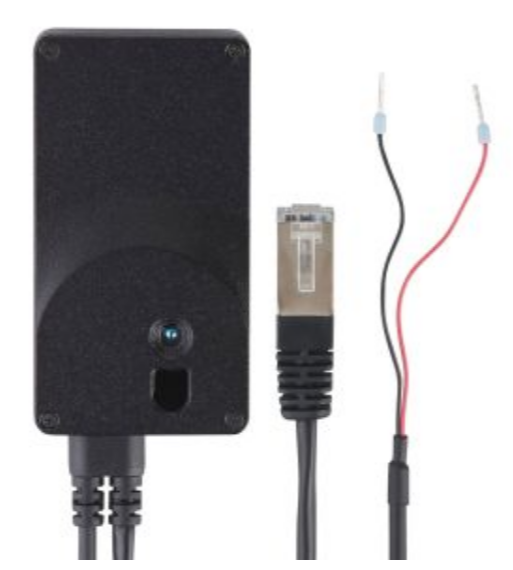
\includegraphics[width=0.4\textwidth]{images/ifm03X100.png}
    \caption{ifm 03X100.}
    \label{fig:ifm03X100}
\end{figure}
\begin{labeling}{\textbf{Field of View    }}
    \setlength{\itemindent}{2em}
    \item [\textbf{Range}] 0.05-3 m
    \item [\textbf{Field of View}] 65Hx45V
    \item [\textbf{Resolution}] 224x172 (20 Hz)
    \item [\textbf{Dimensions}] 80x43,5x21 mm
    \item [\textbf{Connectivity}] Ethernet 10Base-T, 100Base-TX
    \item [\textbf{Driver}] Via PC with ifm Vision Assistant or XML-RPC
    \item [\textbf{Technology}] Time of Flight
    \item [\textbf{Notes}] \textbf{ifm} has \emph{many} cameras on its product line. Some have larger resolution but tighter ranges, for instance. The example shown is one considered a middle point.
\end{labeling}
%%%%%%%%%%%%%%%%%%%%%%%%%%%%%%%%%%%%%%%%%%
\vspace{1em}
\paragraph{\large \textbf{Stereolabs}} {\large ZED2}

\noindent\rule{8cm}{0.1pt}
\begin{figure}[H]
    \centering
    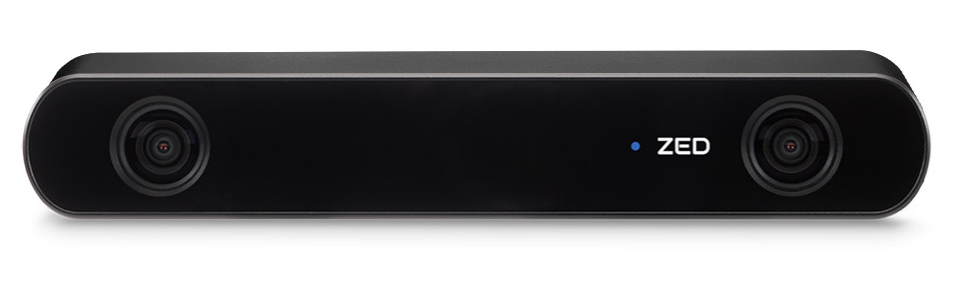
\includegraphics[width=0.5\textwidth]{images/zed2.png}
    \caption{Stereolabs ZED2.}
    \label{fig:zed2}
\end{figure}
\begin{labeling}{\textbf{Field of View    }}
    \setlength{\itemindent}{2em}
    \item [\textbf{Range}] 0.2 - 20 m
    \item [\textbf{Field of View}] 110Hx70V
    \item [\textbf{Resolution}] 1344x376 (up to 100 Hz), 720p (up to 60 Hz), 1080p (up to 30 Hz)
    \item [\textbf{Dimensions}] 175x30x33 mm
    \item [\textbf{Connectivity}] USB 3.0/2.0 Type C
    \item [\textbf{Driver}] ZED SDK with C++ and Python APi and integrated in other frameworks like ROS\footnote{The Robot Operating System (ROS) \cite{ROS_cite}.} and others
    \item [\textbf{Technology}] Stereoscopic vision
\end{labeling}
%%%%%%%%%%%%%%%%%%%%%%%%%%%%%%%%%%%%%%%%%%
\vspace{1em}
\paragraph{\large \textbf{Stereolabs}} {\large ZED Mini}

\noindent\rule{8cm}{0.1pt}
\begin{figure}[H]
    \centering
    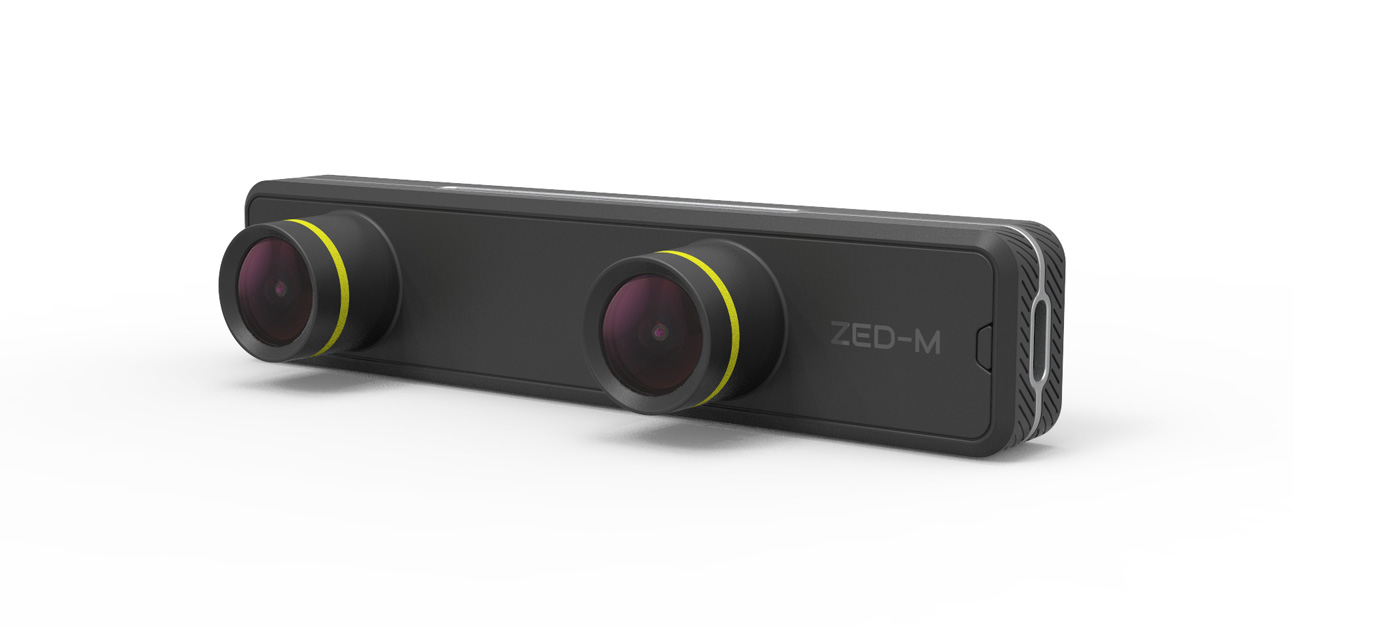
\includegraphics[width=0.6\textwidth]{images/zed-mini.jpg}
    \caption{Stereolabs ZED Mini.}
    \label{fig:zed_mini}
\end{figure}
\begin{labeling}{\textbf{Field of View    }}
    \setlength{\itemindent}{2em}
    \item [\textbf{Range}] 0.1 - 15 m
    \item [\textbf{Field of View}] 90Hx60V
    \item [\textbf{Resolution}] 1344x376 (up to 100 Hz), 720p (up to 60 Hz), 1080p (up to 30 Hz)
    \item [\textbf{Dimensions}] 124.5x30.5x26.5 mm
    \item [\textbf{Connectivity}] USB 3.0/2.0 Type C
    \item [\textbf{Driver}] ZED SDK with C++ and Python APi and integrated in other frameworks like ROS and others
    \item [\textbf{Technology}] Stereoscopic vision
\end{labeling}
%%%%%%%%%%%%%%%%%%%%%%%%%%%%%%%%%%%%%%%%%%
\vspace{1em}
\paragraph{\large \textbf{Carnegie Robotics}} {\large MultiSense S7}

\noindent\rule{8cm}{0.1pt}
\begin{figure}[H]
    \centering
    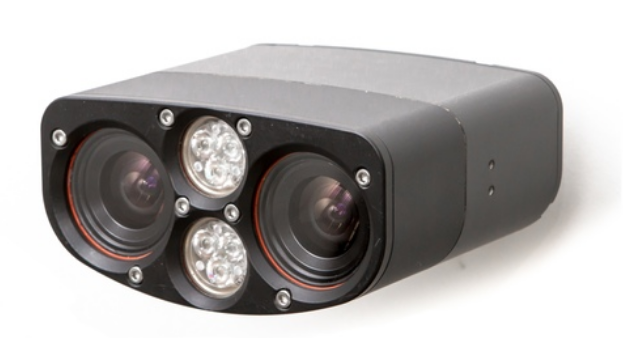
\includegraphics[width=0.5\textwidth]{images/multisenseS7.png}
    \caption{Carnegie Robotics' MultiSense S7.}
    \label{fig:multisenseS7}
\end{figure}
\begin{labeling}{\textbf{Field of View    }}
    \setlength{\itemindent}{2em}
    \item [\textbf{Range}] 0.4 - N/A m
    \item [\textbf{Field of View}] 80Hx45V
    \item [\textbf{Resolution}] 2048x1088 (15 Hz)
    \item [\textbf{Dimensions}] 130x130x65 mm
    \item [\textbf{Connectivity}] Gigabit Ethernet
    \item [\textbf{Driver}] Open source C++ library
    \item [\textbf{Technology}] Stereoscopic vision
\end{labeling}
%%%%%%%%%%%%%%%%%%%%%%%%%%%%%%%%%%%%%%%%%%
\vspace{1em}
\paragraph{\large \textbf{e-con Systems}} {\large TaraXL}

\noindent\rule{8cm}{0.1pt}
\begin{figure}[H]
    \centering
    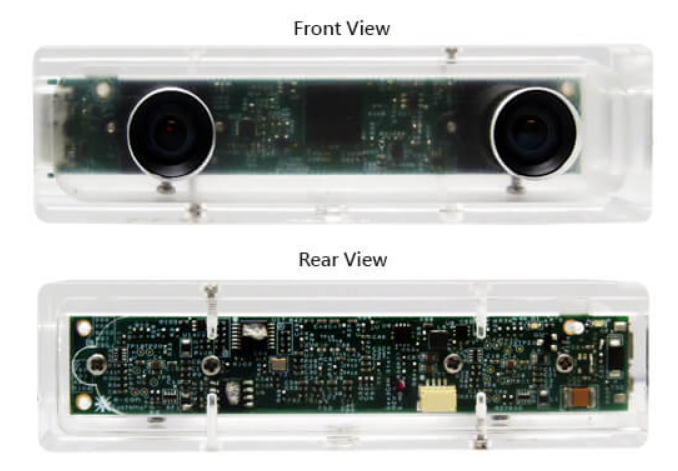
\includegraphics[width=0.5\textwidth]{images/TaraXL.png}
    \caption{e-con Systems' TaraXL.}
    \label{fig:TaraXL}
\end{figure}
\begin{labeling}{\textbf{Field of View    }}
    \setlength{\itemindent}{2em}
    \item [\textbf{Range}] 0.5 - 3 m
    \item [\textbf{Field of View}] N/A
    \item [\textbf{Resolution}] 752x480 (30-60 Hz)
    \item [\textbf{Dimensions}] 100x30x35 mm
    \item [\textbf{Connectivity}] USB 3.0 Type A
    \item [\textbf{Driver}] SDK is built on top of OpenCV 3.4.2 and CUDA
    \item [\textbf{Technology}] Stereoscopic vision
\end{labeling}
%%%%%%%%%%%%%%%%%%%%%%%%%%%%%%%%%%%%%%%%%%
\vspace{1em}
\paragraph{\large \textbf{nerian}} {\large Karmin 3 + SceneScan Pro}

\noindent\rule{8cm}{0.1pt}
\begin{figure}[H]
    \centering
    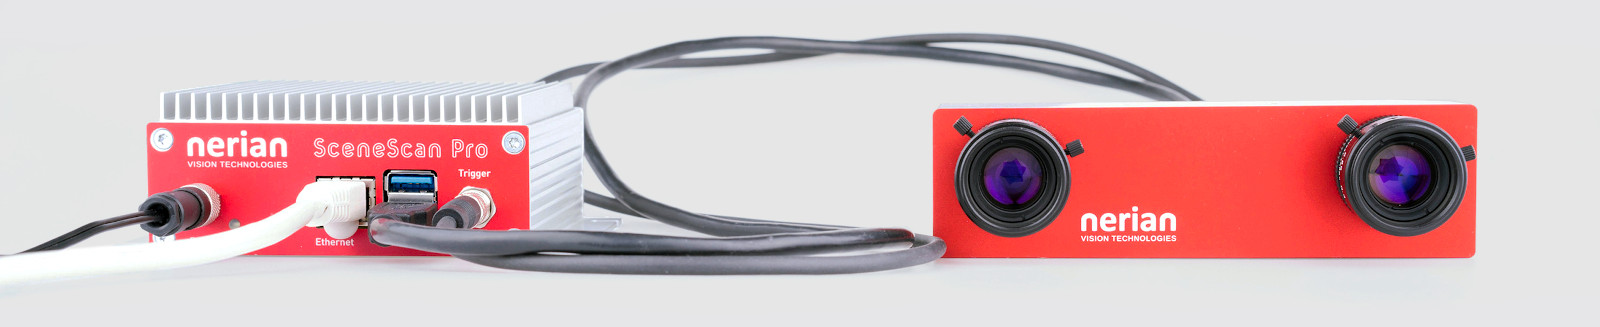
\includegraphics[width=0.9\textwidth]{images/karmin3.jpg}
    \caption{nerian Karmin 3 3D camera.}
    \label{fig:karmin3}
\end{figure}
\begin{labeling}{\textbf{Field of View    }}
    \setlength{\itemindent}{2em}
    \item [\textbf{Range}] 0.2 - N/A
    \item [\textbf{Field of View}] N/A
    \item [\textbf{Resolution}] 1024x768 (30 Hz)
    \item [\textbf{Dimensions}] 144x41x35 mm
    \item [\textbf{Connectivity}] USB 3.0 host, gigabit ethernet
    \item [\textbf{Driver}] \emph{libvisiontransfer}, and API for C++ and Python
    \item [\textbf{Technology}] Stereoscopic vision
    \item [\textbf{Notes}] Karmin 3 has 3 models with 3 different focal distances, depending on the range of operation. The one shown here has 5 cm between sensors, which provides the shortest operating range.
\end{labeling}
%%%%%%%%%%%%%%%%%%%%%%%%%%%%%%%%%%%%%%%%%%
\vspace{1em}
\paragraph{\large \textbf{Framos}} {\large D435e}

\noindent\rule{8cm}{0.1pt}
\begin{figure}[H]
    \centering
    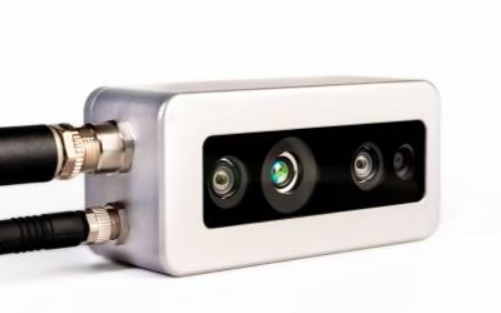
\includegraphics[width=0.5\textwidth]{images/framos.png}
    \caption{The Framos D435e.}
    \label{fig:framos}
\end{figure}
\begin{labeling}{\textbf{Field of View    }}
    \setlength{\itemindent}{2em}
    \item [\textbf{Range}] 0.2 - 10 m
    \item [\textbf{Field of View}] 86Hx57V
    \item [\textbf{Resolution}] 1280x720 (30 Hz)
    \item [\textbf{Dimensions}] 108x24.5x12.5 mm
    \item [\textbf{Connectivity}] Ethernet M12 connector, GigEVision interface
    \item [\textbf{Driver}] Intel RealSense SDK (with bindings for several languages)
    \item [\textbf{Technology}] Stereoscopic vision
    \item [\textbf{Notes}] This is the industrial grade version of the Intel RealSense D435, with a water and dust (IP66) resistant housing, developed by Framos.
\end{labeling}
%%%%%%%%%%%%%%%%%%%%%%%%%%%%%%%%%%%%%%%%%%
\vspace{1em}
\paragraph{\large \textbf{ORBBEC}} {\large Astra Mini}

\noindent\rule{8cm}{0.1pt}
\begin{figure}[H]
    \centering
    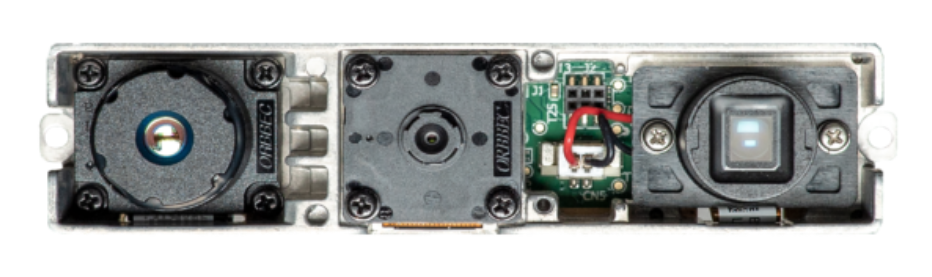
\includegraphics[width=0.5\textwidth]{images/astra_mini.png}
    \caption{Astra Mini from Orbbec.}
    \label{fig:astra_mini}
\end{figure}
\begin{labeling}{\textbf{Field of View    }}
    \setlength{\itemindent}{2em}
    \item [\textbf{Range}] 0.6 - 5 m
    \item [\textbf{Field of View}] 60Hx49V
    \item [\textbf{Resolution}] 640x480 (30 Hz)
    \item [\textbf{Dimensions}] 80x20x20 mm
    \item [\textbf{Connectivity}] USB2.0 (custom cable)
    \item [\textbf{Driver}] Astra SDK
    \item [\textbf{Technology}] Stereoscopic vision
\end{labeling}
%%%%%%%%%%%%%%%%%%%%%%%%%%%%%%%%%%%%%%%%%%
\vspace{1em}
\paragraph{\large \textbf{ORBBEC}} {\large Astra Strereo S U3}

\noindent\rule{8cm}{0.1pt}
\begin{figure}[H]
    \centering
    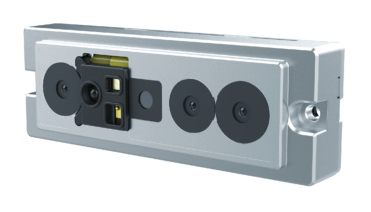
\includegraphics[width=0.4\textwidth]{images/astra_su3.png}
    \caption{Astra S U3 from Orbbec.}
    \label{fig:astra_mini}
\end{figure}
\begin{labeling}{\textbf{Field of View    }}
    \setlength{\itemindent}{2em}
    \item [\textbf{Range}] 0.25-2.5m
    \item [\textbf{Field of View}] 67.9Hx45.3V
    \item [\textbf{Resolution}] 1280×800 (30 Hz), 640×400 (60 Hz), 640×400 (30 Hz)
    \item [\textbf{Dimensions}] 65.3x22.50x12.30 mm
    \item [\textbf{Connectivity}] USB3.0 Type C
    \item [\textbf{Driver}] Astra SDK
    \item [\textbf{Technology}] Stereoscopic vision
\end{labeling}
%%%%%%%%%%%%%%%%%%%%%%%%%%%%%%%%%%%%%%%%%%
\vspace{1em}
\paragraph{\large \textbf{Photoneo}} {\large PhoXi 3D Scanner M}

\noindent\rule{8cm}{0.1pt}
\begin{figure}[H]
    \centering
    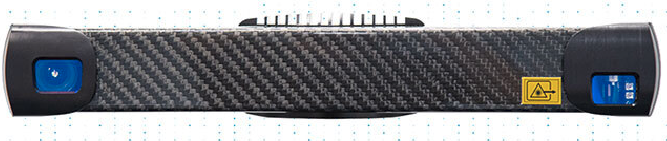
\includegraphics[width=0.5\textwidth]{images/phoXiM.png}
    \caption{PhoXi M 3D Scanner.}
    \label{fig:phoXiM}
\end{figure}
\begin{labeling}{\textbf{Field of View    }}
    \setlength{\itemindent}{2em}
    \item [\textbf{Range}] 0.458-1.118 m
    \item [\textbf{Field of View}] N/A
    \item [\textbf{Resolution}] 3.2 million points
    \item [\textbf{Dimensions}] 77x68x296 mm
    \item [\textbf{Connectivity}] Ethernet with RJ45 socket
    \item [\textbf{Driver}] Pho Xi Control API
    \item [\textbf{Technology}] Stereoscopic vision
\end{labeling}
%%%%%%%%%%%%%%%%%%%%%%%%%%%%%%%%%%%%%%%%%%
\vspace{1em}
\paragraph{\large \textbf{Photoneo}} {\large PhoXi 3D Scanner S}

\noindent\rule{8cm}{0.1pt}
\begin{figure}[H]
    \centering
    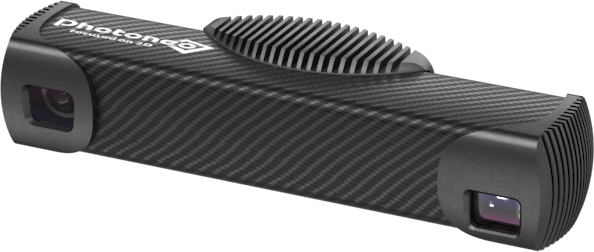
\includegraphics[width=0.4\textwidth]{images/phoXiS.png}
    \caption{PhoXi S 3D Scanner.}
    \label{fig:phoXiS}
\end{figure}
\begin{labeling}{\textbf{Field of View    }}
    \setlength{\itemindent}{2em}
    \item [\textbf{Range}] 0.384-0.52 m
    \item [\textbf{Field of View}] N/A
    \item [\textbf{Resolution}] 3.2 million points
    \item [\textbf{Dimensions}] 77x68x416 mm
    \item [\textbf{Connectivity}] Ethernet with RJ45 socket
    \item [\textbf{Driver}] Pho Xi Control API
    \item [\textbf{Technology}] Stereoscopic vision
\end{labeling}
%%%%%%%%%%%%%%%%%%%%%%%%%%%%%%%%%%%%%%%%%%
\vspace{1em}
\paragraph{\large \textbf{Roboception}} {\large rc\_visard 65 color}

\noindent\rule{8cm}{0.1pt}
\begin{figure}[H]
    \centering
    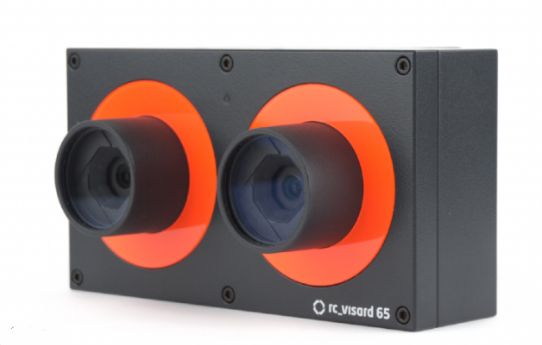
\includegraphics[width=0.3\textwidth]{images/rc_visard65.png}
    \caption{RC Visard 65 3D Scanner.}
    \label{fig:rc_visard65}
\end{figure}
\begin{labeling}{\textbf{Field of View    }}
    \setlength{\itemindent}{2em}
    \item [\textbf{Range}] 0.2 - 1 m
    \item [\textbf{Field of View}] 61Hx48V
    \item [\textbf{Resolution}] 1280x960 (0.8 Hz), 640x480 (3 Hz), 320x240 (15 Hz),
    214x160 (25 Hz)
    \item [\textbf{Dimensions}] 135x75x96 mm
    \item [\textbf{Connectivity}] M12 8-pin Ethernet socket connector
    \item [\textbf{Driver}] They provide a Web Interface, Rest-API, ROS and GenICam
    \item [\textbf{Technology}] Stereoscopic vision
    \item [\textbf{Notes}] IP54 protective casing
\end{labeling}
%%%%%%%%%%%%%%%%%%%%%%%%%%%%%%%%%%%%%%%%%%
\vspace{1em}
\paragraph{\large \textbf{Zivid}} {\large One+ Small}

\noindent\rule{8cm}{0.1pt}
\begin{figure}[H]
    \centering
    \includegraphics[width=0.4\textwidth]{images/ZividOneSmall.jpg}
    \caption{Zivid One+ Small 3D Scanner.}
    \label{fig:ZividOneSmall}
\end{figure}
\begin{labeling}{\textbf{Field of View    }}
    \setlength{\itemindent}{2em}
    \item [\textbf{Range}] 300-800 mm 
    \item [\textbf{Field of View}] 164x132 mm at 0.3 m and 621x439 mm at 1.0 m
    \item [\textbf{Resolution}] 1920x1200
    \item [\textbf{Dimensions}] 226x86x165 mm
    \item [\textbf{Connectivity}] USB3.0 Type B
    \item [\textbf{Driver}] Zivid SDK, with bindings for many languages, and integrates with ROS
    \item [\textbf{Technology}] Structured Light
    \item [\textbf{Notes}] IP65 protective casing
\end{labeling}
%%%%%%%%%%%%%%%%%%%%%%%%%%%%%%%%%%%%%%%%%%
\vspace{1em}
\paragraph{\large \textbf{Microsoft}} {\large Kinect v2}

\noindent\rule{8cm}{0.1pt}
\begin{figure}[H]
    \centering
    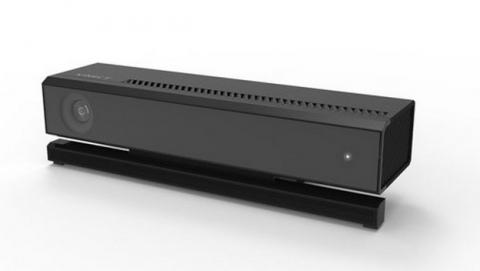
\includegraphics[width=0.5\textwidth]{images/kinect2.jpg}
    \caption{Kinect 2 sensor from Microsoft.}
    \label{fig:kinect2}
\end{figure}
\begin{labeling}{\textbf{Field of View    }}
    \setlength{\itemindent}{2em}
    \item [\textbf{Range}] 300-800 mm 
    \item [\textbf{Field of View}] 70.6Hx60V
    \item [\textbf{Resolution}] 512x424
    \item [\textbf{Dimensions}] 66x249x67 mm
    \item [\textbf{Connectivity}] USB3.0 Type B
    \item [\textbf{Driver}] Kinect SDK 2.0 for Windows (other non-official SDKs for Linux exist too)
    \item [\textbf{Technology}] Time of Flight
    \item [\textbf{Notes}] It is in the process of being discontinued (although it can still be purchased from retailers), but is presented here due to its importance in the industry back when it was released in 2014. It was first designed for the Xbox One console as an accessory, and later converted as a development kit.
\end{labeling}
%%%%%%%%%%%%%%%%%%%%%%%%%%%%%%%%%%%%%%%%%%
\vspace{1em}
\paragraph{\large \textbf{Basler}} {\large Blaze ToF camera}

\noindent\rule{8cm}{0.1pt}
\begin{figure}[H]
    \centering
    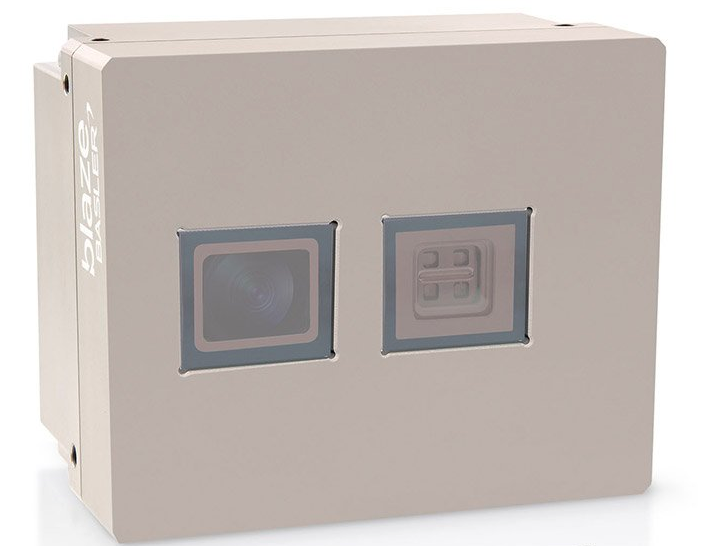
\includegraphics[width=0.3\textwidth]{images/basler_blaze_tof.png}
    \caption{Basler Blaze 3D camera.}
    \label{fig:basler_blaze_tof}
\end{figure}
\begin{labeling}{\textbf{Field of View    }}
    \setlength{\itemindent}{2em}
    \item [\textbf{Range}] 0-10 m
    \item [\textbf{Field of View}] 60Hx45V
    \item [\textbf{Resolution}] 640x480 (30 Hz)
    \item [\textbf{Dimensions}] 99.6x80.6x67.9 mm
    \item [\textbf{Connectivity}] M12 GigE cable
    \item [\textbf{Driver}] Blaze SDK C++ API, has easy integration with frameworks like PCL or ROS
    \item [\textbf{Technology}] Time of Flight
    \item [\textbf{Notes}] Monochrome, not color
\end{labeling}
%%%%%%%%%%%%%%%%%%%%%%%%%%%%%%%%%%%%%%%%%%
\vspace{1em}
\paragraph{\large \textbf{Mynt}} {\large Eye S210}

\noindent\rule{8cm}{0.1pt}
\begin{figure}[H]
    \centering
    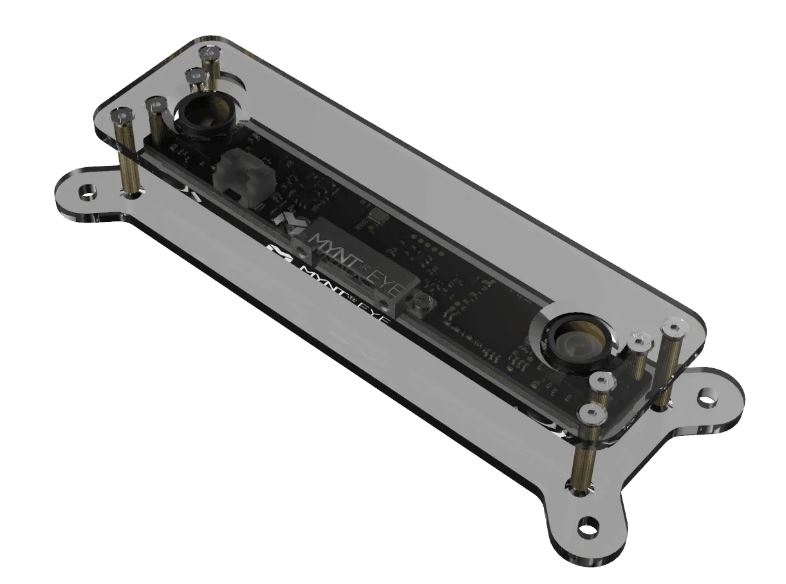
\includegraphics[width=0.5\textwidth]{images/MinteyeS210.png}
    \caption{Mynt Eye S210 3D camera.}
    \label{fig:MinteyeS210}
\end{figure}
\begin{labeling}{\textbf{Field of View    }}
    \setlength{\itemindent}{2em}
    \item [\textbf{Range}] 0.5-7 m
    \item [\textbf{Field of View}] 95Hx50V
    \item [\textbf{Resolution}] 1280x400 (60 Hz) or 2560x800 (30 Hz)
    \item [\textbf{Dimensions}] 125x47x26.6 mm 
    \item [\textbf{Connectivity}] USB 3.0
    \item [\textbf{Driver}] Mynt Eye SDK in C++
    \item [\textbf{Technology}] Stereoscopic vision
    \item [\textbf{Notes}] Has Inertia Measurement Unit (IMU)
\end{labeling}
%%%%%%%%%%%%%%%%%%%%%%%%%%%%%%%%%%%%%%%%%%
\vspace{1em}
\paragraph{\large \textbf{Mynt}} {\large Eye D-1000-120}

\noindent\rule{8cm}{0.1pt}
\begin{figure}[H]
    \centering
    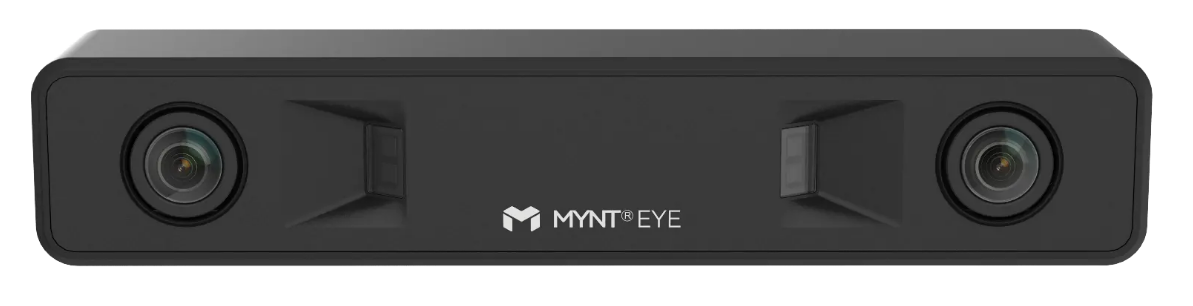
\includegraphics[width=0.5\textwidth]{images/MinteyeD1000120.png}
    \caption{Mynt Eye S210 3D camera.}
    \label{fig:MinteyeD1000120}
\end{figure}
\begin{labeling}{\textbf{Field of View    }}
    \setlength{\itemindent}{2em}
    \item [\textbf{Range}] 0.3-10 m
    \item [\textbf{Field of View}] 105Hx58V
    \item [\textbf{Resolution}] 1280x400 (60 Hz) or 2560x800 (30 Hz)
    \item [\textbf{Dimensions}] 165x30x30 mm 
    \item [\textbf{Connectivity}] USB 3.0   
    \item [\textbf{Driver}] Mynt Eye SDK in C++
    \item [\textbf{Technology}] Stereoscopic vision
    \item [\textbf{Notes}] Has Inertia Measurement Unit (IMU)
\end{labeling}
%%%%%%%%%%%%%%%%%%%%%%%%%%%%%%%%%%%%%%%%%%
\vspace{1em}
\paragraph{\large \textbf{pmdtec}} {\large Camboard pico flexx}

\noindent\rule{8cm}{0.1pt}
\begin{figure}[H]
    \centering
    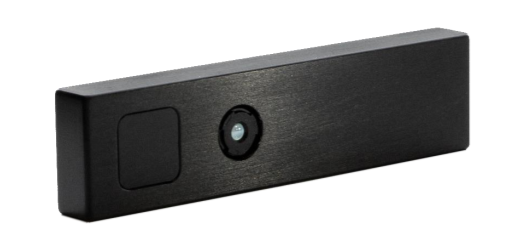
\includegraphics[width=0.5\textwidth]{images/camboardPicoFlexx.png}
    \caption{Camboard pico flexx 3D camera from pmd tech.}
    \label{fig:camboardPicoFlexx}
\end{figure}
\begin{labeling}{\textbf{Field of View    }}
    \setlength{\itemindent}{2em}
    \item [\textbf{Range}] 0.1-4 m
    \item [\textbf{Field of View}] 62Hx45V
    \item [\textbf{Resolution}] 224x171 (45 Hz)
    \item [\textbf{Dimensions}] 68x17x7.35 mm
    \item [\textbf{Connectivity}] USB 2.0 Micro B 
    \item [\textbf{Driver}] Royale SDK in C++, and supports frameworks like ROS, OpenCV, etc
    \item [\textbf{Technology}] Time of Flight
\end{labeling}
%%%%%%%%%%%%%%%%%%%%%%%%%%%%%%%%%%%%%%%%%%
\vspace{1em}
\paragraph{\large \textbf{Hokuyo}} {\large Scanning Rangefinder UST-10LX}

\noindent\rule{8cm}{0.1pt}
\begin{figure}[H]
    \centering
    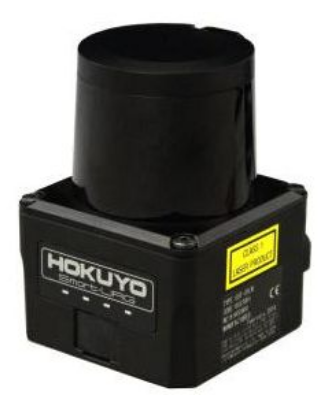
\includegraphics[width=0.3\textwidth]{images/HokuyoUST10LX.png}
    \caption{UST-10LX LiDAR sensor from Hokuyo.}
    \label{fig:HokuyoUST10LX}
\end{figure}
\begin{labeling}{\textbf{Field of View    }}
    \setlength{\itemindent}{2em}
    \item [\textbf{Range}] 0.06-10 m
    \item [\textbf{Field of View}] 270H
    \item [\textbf{Resolution}] 0.25 angular (40 Hz)
    \item [\textbf{Dimensions}] 50x50x70 mm
    \item [\textbf{Connectivity}] Ethernet 100BASE-TX
    \item [\textbf{Driver}] Sensor Communication Protocol (SCIP)
    \item [\textbf{Technology}] LiDAR
    \item [\textbf{Notes}] IP 67 protective casing
\end{labeling}
%%%%%%%%%%%%%%%%%%%%%%%%%%%%%%%%%%%%%%%%%%
\vspace{1em}
\paragraph{\large \textbf{Intel}} {\large RealSense L515}

\noindent\rule{8cm}{0.1pt}
\begin{figure}[H]
    \centering
    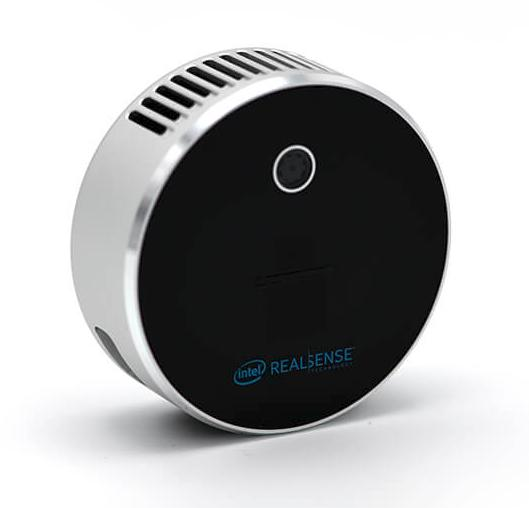
\includegraphics[width=0.3\textwidth]{images/realsenseL515.jpg}
    \caption{Intel RealSense L515 LiDAR 3D camera.}
    \label{fig:realsenseL515}
\end{figure}
\begin{labeling}{\textbf{Field of View    }}
    \setlength{\itemindent}{2em}
    \item [\textbf{Range}] 0.25-9 m
    \item [\textbf{Field of View}] 70Hx55V
    \item [\textbf{Resolution}] 1024x768 (30 Hz)
    \item [\textbf{Dimensions}] 61 mm diameter × 26 mm height
    \item [\textbf{Connectivity}] USB3.1 Type C
    \item [\textbf{Driver}] RealSense SDK (with bindings for many languages, like Python and C++)
    \item [\textbf{Technology}] LiDAR
\end{labeling}
%%%%%%%%%%%%%%%%%%%%%%%%%%%%%%%%%%%%%%%%%%
\vspace{1em}
\paragraph{\large \textbf{Intel}} {\large RealSense D435}

\noindent\rule{8cm}{0.1pt}
\begin{figure}[H]
    \centering
    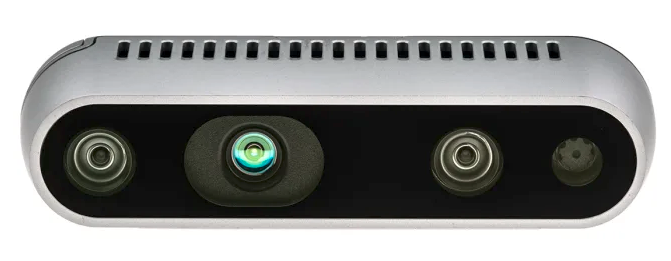
\includegraphics[width=0.5\textwidth]{images/realsenseD435.png}
    \caption{Intel RealSense D435 3D camera.}
    \label{fig:realsenseD435}
\end{figure}
\begin{labeling}{\textbf{Field of View    }}
    \setlength{\itemindent}{2em}
    \item [\textbf{Range}] 0.105-10 m
    \item [\textbf{Field of View}] 85Hx58V
    \item [\textbf{Resolution}] 1280x720 (30 Hz)
    \item [\textbf{Dimensions}] 99x25x25 mm
    \item [\textbf{Connectivity}] USB3.0 Type C
    \item [\textbf{Driver}] RealSense SDK (with binding for many languages, like Python and C++)
    \item [\textbf{Technology}] Stereoscopic vision
    \item [\textbf{Notes}] Intel has a range of cameras like this one, suited for different ranges and some integrate an IMU (but not this one)
\end{labeling}
%%%%%%%%%%%%%%%%%%%%%%%%%%%%%%%%%%%%%%%%%%



%%%%%%%%%%%%%%%%%%%%% END CAMERA LISTING %%%%%%%%%%%%%%%%%%%%%

\subsubsection{The Realsense D435}
From the list of cameras shown earlier, the one chosen is the Intel RealSense D435. There are many important aspects that need to be taken into account when it comes to choosing a specific depth camera:
\begin{enumerate}
    \item \textbf{Range}. The camera, as mentioned, should not be further than 1 meter from the testbench, but there is no limit in how close it can be from it. Hence, the minimum range of the camera must be as small as possible.
    \item \textbf{Depth resolution}. How much resolution (and field of view) the depth sensor of the camera has will determine how much detail can the later point cloud have. The larger, the better. Since there are no real-time requirements for this thesis, the frames per second the camera can process are of no relevance, which in general allows for the largest resolutions. The cameras based on Time of Flight technology have, as it can be observed, the lowest resolutions, so they are discarded. 
    \item \textbf{RGB capability}. Although the majority, not all cameras listed can generate both a depth image and an RGB image at the same time. This is crucial to be able to combine object detection approaches that leverage both 2D and 3D information, as well as to create colored point clouds.
    \item \textbf{A good Standard Development Kit (SDK)}. Where most time can be spent is in communicating with the camera from the PC. Almost all camera manufacturers provide Standard Development Kits that ease this task with relatively simple code, provided one reads the docs. There is no guarantee that an SDK will actually be user-friendly until it is tested in situ, but popularity online is a good measure (both by positive opinions and number of entries in Q\&A sites).
    \item \textbf{Price}. Need not be explained the importance of a reasonable price, specially given the fact that this is an academic project. Objects just need to be scanned with a quality good enough to visually identify them, and not in a photorealistic manner. Hence, prices for entry-level products should not go beyond 400 euros.
\end{enumerate}
From the aspects mentioned in the list above the Intel RealSense D435 is considered as the best all-around choice. 

\subsubsection{Using the RealSense SDK} \label{sec:using_realsense_sdk}
The Intel RealSense division has put many resources into producing a unified Standard Development Kit for all RealSense cameras, that is easy to use and with bindings in the most popular languages. For this thesis the C++ client has been used (the actual language with which the SDK is built) in conjunction with OpenCV and PCL. With the help of the code samples in RealSense's website\footnote{\url{https://dev.intelrealsense.com/docs/code-samples?_ga=2.191648938.1238222063.1623263754-1998510554.1614708955}} a small app is built to stream real time point cloud data (created in real time with the depth image provided by the camera) and RGB video. The app is designed to listen for key presses, specifically the `s' and `Space bar' keys. The latter recenters the camera when visualizing the point cloud and the former saves the point cloud and RGB image to disk. The RGB image is saved as a `.png', and the point cloud in `.pcd' format. The `.pcd' format is the default point cloud format defined by the PCL library, and since it is used extensively and provides input/output tools, makes sense to use it. Figure \ref{fig:realsense_SDK_1} is the app running, with each window displaying the RGB image and RGB point cloud stream from the camera. The viewpoint of the point cloud can be changed from the initial position by clicking and dragging with the mouse, as can be observed in figure \ref{fig:realsense_SDK_rotated}.

It has to be noted that the `.png' RGB image is not the actual one stored in the left viewport of \ref{fig:realsense_SDK_1}. Instead, the image is the colorized depth image, which rather looks like the one of \ref{fig:colored_depth_image}. The colorized depth image is obtained from aligning the depth image and the RGB image.

\begin{figure}[h]
    \centering
    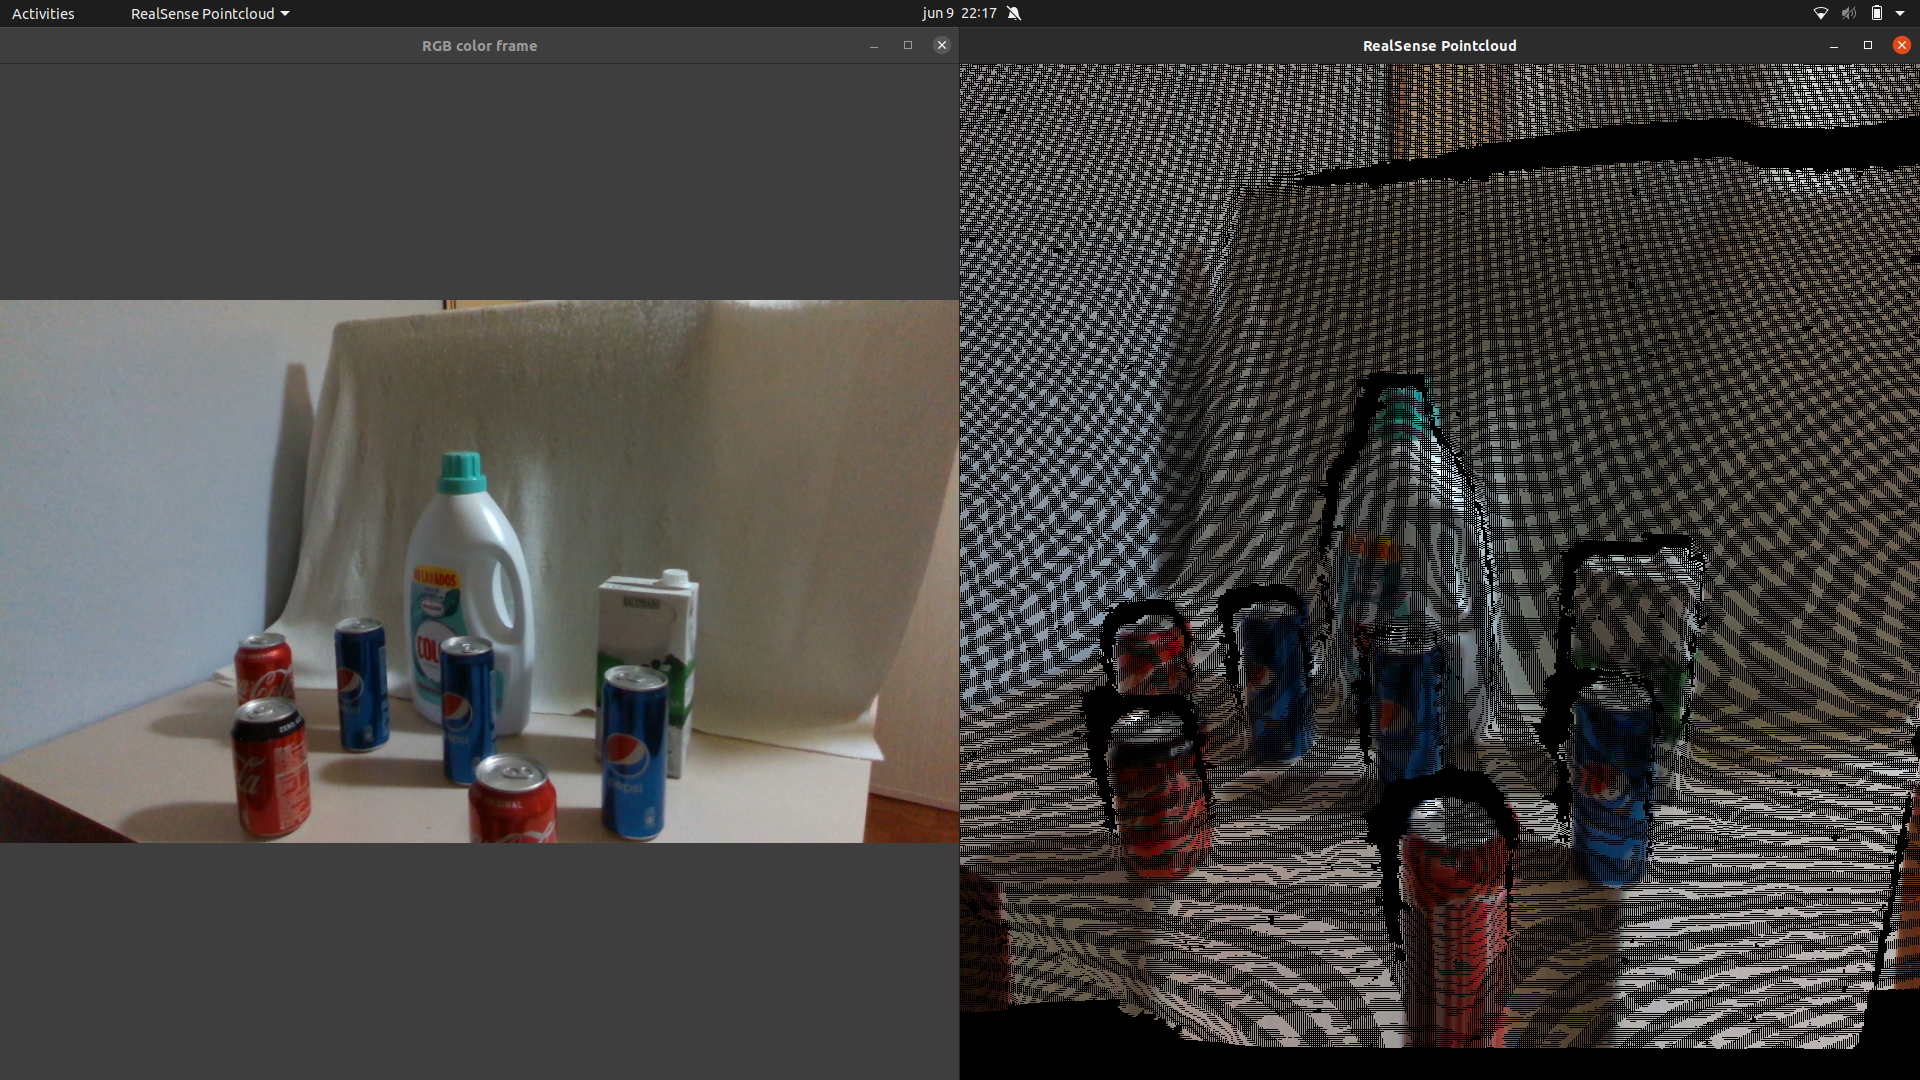
\includegraphics[width=1\linewidth]{images/realsense_SDK_1.png}
    \caption{Screenshot of the app created with the RealSense SDK and OpenCV (and PCL for storing to disk).}
    \label{fig:realsense_SDK_1}
\end{figure}

\begin{figure}[h]
    \centering
    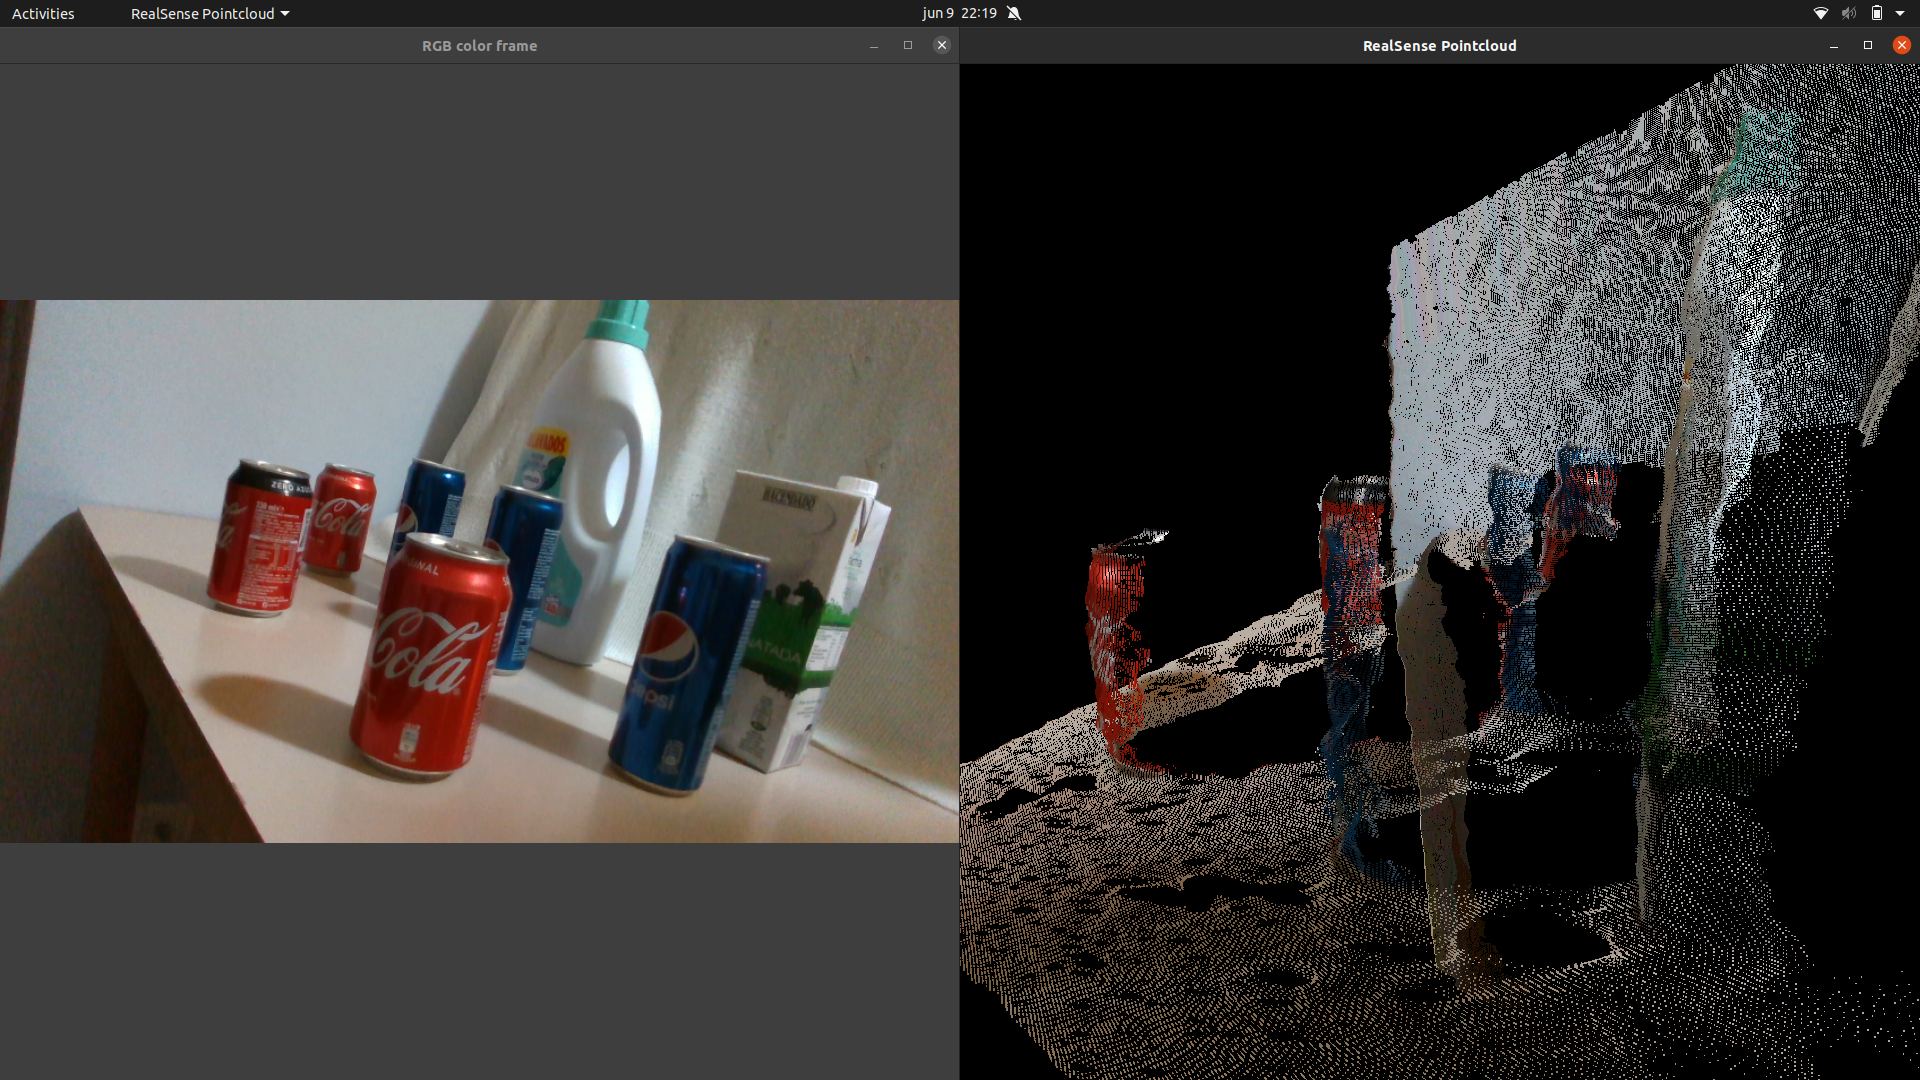
\includegraphics[width=1\linewidth]{images/realsense_SDK_rotated.png}
    \caption{Screenshot of the app with the point cloud's viewport moved with the mouse.}
    \label{fig:realsense_SDK_rotated}
\end{figure}

\begin{figure}[h]
    \centering
    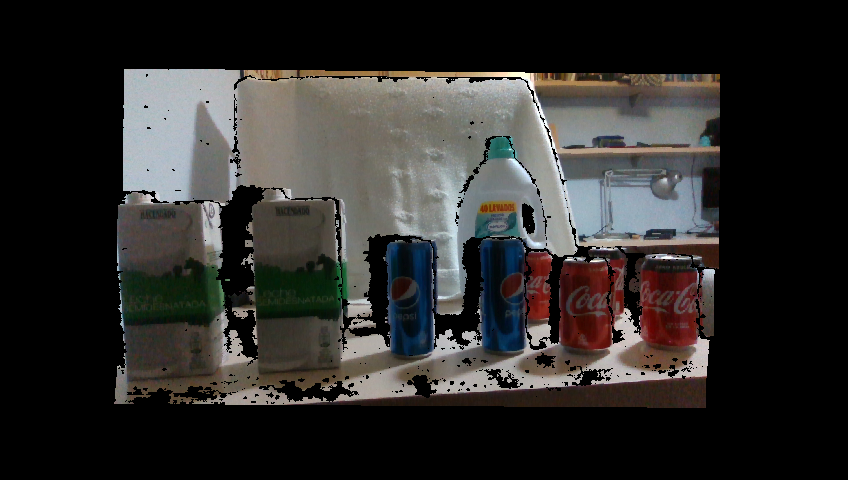
\includegraphics[width=1\linewidth]{images/colored_depth_image.png}
    \caption{Depth image aligned with the RGB image. Artifacts, like zones with no information, are due to the nature of the depth image. Notice how shadows are mainly to the left of the objects: this is because the depth sensor is at the rightmost zone of the camera.}
    \label{fig:colored_depth_image}
\end{figure}

When the user presses the `s' key, a part from storing the `.pcd' and `.png' point cloud and image, a `.json' dictionary is also stored. This dictionary contains intrinsic parameters of the camera, namely:
\begin{itemize}
    \item \emph{fx}: Focal length of the image as a multiple of pixel width.
    \item \emph{fy}: Focal length of the image as a multiple of pixel height.
    \item \emph{height}: Number of columns in the depth image.
    \item \emph{width}: Number of rows in the depth image.
    \item \emph{model}: Which of the distortion models is used (stored as an integer).
    \item \emph{ppx}: Pixel coordinates of the center of projection in $x$.
    \item \emph{ppy}: Pixel coordinates of the center of projection in $y$.
\end{itemize}
The aforementioned parameters will be needed to project points from the point cloud to the `.png' image. In essence, they are the relationship between the 2D and 3D streams' coordinate systems.

\subsection{Frameworks and languages}
This section is designed to introduce the languages and frameworks that will be used all throughout the project and provide some reasoning on why they are used, as well as to provide some background in the array of options out there and why ones are chosen above others. Since most of the concepts of this work are yet to be introduced in the upcoming sections I will try to gently introduce and reference the frameworks this section will describe as they go.

This work is based on a dual approach to the concept of computer vision\footnote{Taking the meaning of \emph{computer vision} in the broadest sense possible, that is, making machines sense the environment, irrespective of how the environment is recorded.}: 2D digital image processing (in the form of bitmaps) and 3D point cloud processing. Hence, it makes sense to assess the capabilities of the most important libraries that tackle those tasks.

\paragraph{Most prominent 2D image processing libraries} 
There are many image processing libraries. However, only the most notable ones are listed here. The newest machine/deep learning libraries, although used extensively for computer vision-related tasks, are not included in this list but rather given a dedicated chapter later on.
\begin{itemize}
    \item OpenCV: the Open Source Computer Vision library was started in 1999 by an Intel Research member called Gary Bradski, with the aim of making computer vision universally available. Its developing team has changed with time, but receives periodic improvements from the computer vision community. So much so that it incorporates some Deep Learning algorithms. OpenCV was built from the start with optimization and real-time applications in mind, making its algorithms as fast they can go. On top of that, it uses hardware acceleration\footnote{Like SIMD instruction sets.} when it can. Its interfaces are C++ (the language in which it is written), Python, Java and MATLAB, which is very useful when incorporating OpenCV into existing code bases not necessarily written in C++. The fact that the interface supports higher-level languages like Python (via Python bindings created using the Python/C API\footnote{\url{https://docs.python.org/3/c-api/index.html}}) makes writing programs fast and enhances productivity by being able to use widely popular packages like Numpy, Matplotlib, and others.
    
    OpenCV is the go-to library for image processing (so much so that, at the time of writing, their webpage states 18 million downloads), so the newest algorithms in the literature tend to be implemented first there, either by the same author or people who understood them. This and the fact that it is a 20+ year old library makes it incredibly robust and proof tested.

    The library comes with an Apache 2 license, making it free to distribute, modify and use even for commercial applications (arguably this is one of the driving forces behind its popularity). Patented algorithms implemented in OpenCV, however, are not actually free to use and may require royalties or some kind of fees to the patent holders (like the SIFT algorithm, explained in this project).

    \item Scipy: the Scipy package \cite{scipy_paper} was published in 2001 with the purpose of being a whole ecosystem of open-source tools for mathematics, science and engineering. It being an ecosystem provides a core library on top of supporting other packages like SymPy, NumPy, Matplotlib, and others. In particular, Scipy's core module \texttt{ndimage} supports several image processing related tasks. It has been superseded by Scikit-image.
    \item Scikit-image: the package scikit-image \cite{skimage_paper} is an open source image processing library that derived from Scipy, with the intention to focus on image processing related tasks. It was first released in 2009 and has since undergone a long way of continuous improvements from the community. It does not come with as wide an array of solutions as OpenCV does, but instead provides (1) high quality open and free pythonic code that has been peer reviewed prior to its inclusion in the package; (2) a focus on education; (3) a sufficient range of state of the art algorithms; and (4) efficient code that runs reasonably fast (some sections of the code are written in Cython or use Numba) and uses the de facto standards of Python in the science realm (that is, NumPy and Matplotlib).
\end{itemize}

\paragraph{3D point cloud processing libraries}
There are fewer options regarding the processing of point clouds. OpenCV, although known for its 2D image processing capabilities, has some 3D processing features. But the go-to library is actually the Point Cloud Library (PCL) \cite{pcl_paper}, launched in 2011. Just like OpenCV, it is implemented in C++ with efficiency and speed in mind\footnote{SIMD instruction set for CPU computing and CUDA for GPU computing.}, and includes almost all the latest and greatest algorithms from the literature, either implemented by their own authors or others persons in the community. Despite its popularity, it does not provide an interface other than the C++ API in which it was coded.

The framework of choice for the 2D approach (Section \ref{sec:2D_approach}) is OpenCV, used with the Python bindings. Combining the completeness and robustness of OpenCV with the boost in productivity Python itself as a language offers (compared to C++) and the array of packages that can be used alongside is key to this work. The framework of choice for the 3D approach (Section \ref{sec:3D_approach}) is PCL, again, for its completeness and robustness. Sadly, there are no official Python bindings, which means that all work will need to be carried out with its C++ API and no interaction with the Python interpreter is possible (unless I built custom bindings, which is not feasible due to time constraints). Code from the 3D approach should be self contained, and any interaction using Python would need to be done by firstly writing the data to disk and then reading it again from the other end (from the Python's end that is).

\paragraph{Deep learning frameworks}
Section \ref{sec:world_neural_networks} of this work explores the use of Deep Learning for approaching the object detection issue. Hence, it is pertinent to provide a full comparison of the competitive deep learning frameworks available. It has to be noted that deep learning is a type of approach that works for both 2D images and 3D point cloud data.

\begin{itemize}
    \item TensorFlow:
    \item PyTorch:
    \item MXnet:
\end{itemize}

\paragraph{Essential libraries} 
Python is one of the most popular \cite{TODO:citeTIOBEindex} languages for two main reasons: first, the fact that it is a dynamic\footnote{Meaning it executes in runtime tasks that other languages would do in compile time.} high level language that allows for high productivity; and second because of its ecosystem. Ecosystem meaning the set of quality libraries that surround the language itself and make it ideal for a wide array of tasks. Those libraries are contributed freely by the community, and have become so ubiquitous that are almost considered \emph{de facto} standards, particularly in the scientific computing area. The ones used for this project are listed below:
\begin{enumerate}
    \item NumPy:
    \item Matplotlib:
    \item Numba: TODO:mencionar la sección exacta en la que se usa!
\end{enumerate}

And last but certainly not least, the Python Standard Library, which, as the name suggests, comes with the Python distribution. It offers a wide range of facilities to everyday hassles programmers may encounter, and does so in an OS-independent API manner. Such facilities include I/O functionality, networking, parsing, database management, email handling, and a long etcetera. Full list is provided in the official documentation\footnote{\url{https://docs.python.org/3/library/}}.

% Y LUEGO DE LAS LIBRERÍAS ESENCIALES QUE VAN INCLUIDAS DE FACTO EN EL PROYECTO: NUMPY, MATPLOTLIB, Y EVIDENTEMENTE UN USO INTELIGENTE DE LA LIBRERIA ESTANDAR DE PYTHON

 
\end{document}